
\documentclass{scrreprt}
\usepackage{graphicx}
\usepackage{subcaption}
\usepackage{float}
\usepackage{amsmath}
\usepackage{listings}
\usepackage{color}
\usepackage{tikz}
\usepackage{circuitikz}
\usepackage{url}
\usepackage{xurl}
\usepackage[colorlinks=true, linkcolor=blue]{hyperref}
\usepackage{booktabs}
\usepackage{karnaugh-map}

\title{Assignment 4 \\ Mod 5 Counter \& Band Pass Filter}
\author{Jnanesh Sathisha Karmar - EE25BTECH11029 \\ Vivek Kumar - EE25BTECH11062}
\date{February 14, 2026}

\definecolor{lbcolor}{rgb}{0.96,0.96,0.863} 

\lstset{basicstyle=\ttfamily, keywordstyle=\rmfamily\bfseries, backgroundcolor=\color{lbcolor}}

\begin{document}

\maketitle

\chapter{Mod 5 Counter}

\section{Objective}
Our objective is to build a mod 5 counter (should display 0, 1, 2, 3 and 4) using 3 LEDs. The LEDs represent the state (a number from 0-4) in corresponding binary format. For example, the LED states to represent the number 3 would be OFF, ON and ON. The counter will increment after every clock pulse (just after every rising edge). When the counter reaches 4, it loops back to 0.

\begin{figure}[H]
    \centering
    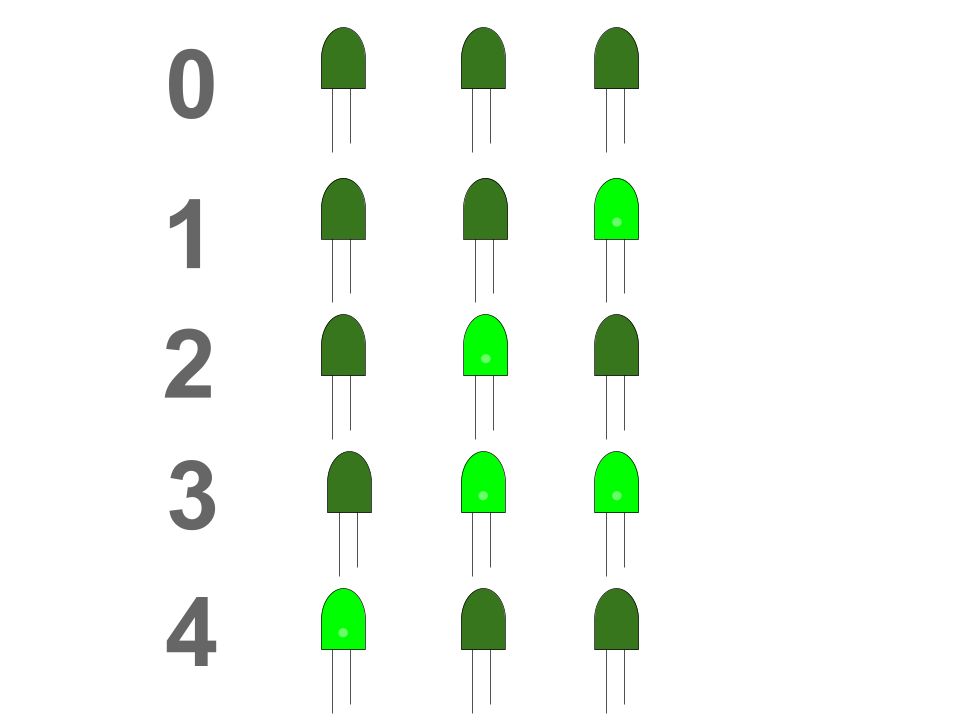
\includegraphics[width=0.5\linewidth]{led-states.png}
    \caption{Representation of counter states}
    \label{fig:led-states}
\end{figure}

\section{Setup}
We can achieve this with the help of three JK Flip-Flops (to store the state), and a few AND and NOR gates. We can use a DC Voltage source or an Arduino UNO to supply 5 Volts DC. We can use an AFG to give clock signal(either by giving a square wave of duty cycle 50\% and frequency 1Hz, or supplying one square pulse through trigger mode). We can also use an Arduino UNO to supply a clock signal (through any one of the digital pins). In this case, we chose a square wave frequency of 1Hz so that we can see the counter increment properly. If we had applied a higher frequency, we would not be able to see or capture the counter state through the LEDs (the LEDs will turn ON and OFF really quick)

The list of exact components required for the Mod 5 counter are given below: 

\begin{itemize}
    \item 3 - 7476 JK FF ICs
    \item 1 - 7408 Quad AND Gate IC
    \item 1 - 7402 Quad NOR Gate IC
\end{itemize}

\section{Logic for Counter}
We can use a state diagram to represent the states the counter goes through.

\begin{figure}[H]
    \centering
    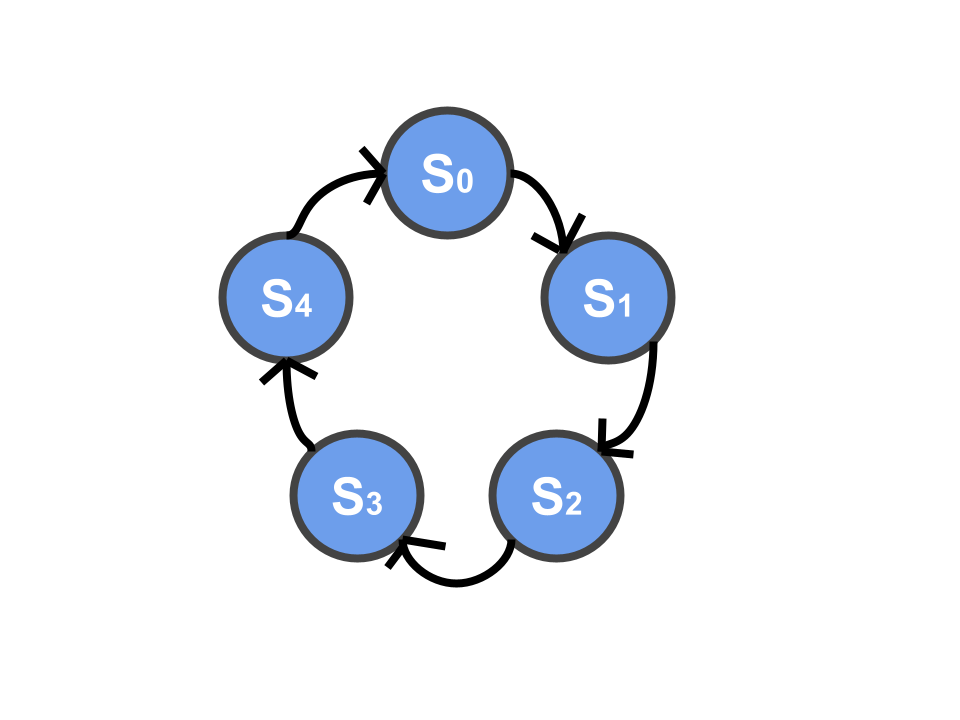
\includegraphics[width=0.6\linewidth]{state-diagram.png}
    \caption{State diagram for mod 5 counter}
    \label{fig:statediagram}
\end{figure}

For the 5 states, we would require 3 Flip-Flops (2 Flip-Flops can represent at-most $2^2 = 4$ states and 3 can represent at-most $2^3 = 8$ states. This is of course by assuming that each state is represented as a binary number starting from 0.

The truth table for achieving this is given below.
\begin{table}[H]
    \centering
    \begin{tabular}{|c|c|c|c|c|c|c|c|c|}
    \hline
         $Q_2$ & $Q_1$ & $Q_0$ & $J_2K_2$ & $J_1K_1$ &$J_0K_0$ & $Q_{new,2}$ & $Q_{new,1}$ & $Q_{new,0}$ \\
    \hline
        0 & 0 & 0 & 0 X & 0 X & 1 X & 0 & 0 & 1 \\
        0 & 0 & 1 & 0 X & 1 X & X 1 & 0 & 1 & 0 \\
        0 & 1 & 0 & 0 X & X 0 & 1 X & 0 & 1 & 1 \\
        0 & 1 & 1 & 1 X & X 1 & X 1 & 1 & 0 & 0 \\
        1 & 0 & 0 & X 1 & 0 X & 0 X & 0 & 0 & 0 \\
        1 & 0 & 1 & X 1 & 0 X & X 1 & 0 & 0 & 0 \\
        1 & 1 & 0 & X 1 & X 1 & 0 X & 0 & 0 & 0 \\
        1 & 1 & 1 & X 1 & X 1 & X 1 & 0 & 0 & 0 \\
    \hline
    \end{tabular}
    \caption{Truth table}
    \label{tab:truthtable}
\end{table}

Here X stands for don't care.

Note that in the above truth table, we made sure that the next Q for undefined states (5,6,7) goes back to 0. This is to ensure that we come back to a defined state even if we start with an undefined state. If we had left the output as don't cares, then it might take a few iterations (or worse, get stuck) to come out of the set of undefined states. 

We can draw K-maps for $J_2, K_2, J_1, K_1, J_0, K_0$, so that we can obtain a simplified expression for the inputs of JK FF :

\begin{minipage}{0.45\textwidth}
\bigskip
\textbf{For} $\mathbf{J_2}$:
\begin{center}
\begin{karnaugh-map}[4][2][1][$Q_0$][$Q_1$][$Q_2$]
    \manualterms{0, 0, 0, 1, X, X ,X, X}
    \implicant{3}{7}
\end{karnaugh-map}
\begin{align}
    J_2 = Q_1Q_0 \label{eq:j2}
\end{align}
\end{center}
\end{minipage}
\hfill
\begin{minipage}{0.45\textwidth}
\bigskip
\textbf{For} $\mathbf{K_2}$:
\begin{center}
\begin{karnaugh-map}[4][2][1][$Q_0$][$Q_1$][$Q_2$]
    \manualterms{X, X, X, X, 1, 1, 1, 1}
    \implicant{0}{6}
\end{karnaugh-map}
\begin{align}
    K_2 = 1 \label{eq:k2}
\end{align}
\end{center}
\end{minipage}

\noindent
\begin{minipage}{0.45\textwidth}
\bigskip
\textbf{For} $\mathbf{J_1}$:
\begin{center}
\begin{karnaugh-map}[4][2][1][$Q_0$][$Q_1$][$Q_2$]
    \manualterms{0, 1, X, X, 0, 0, X, X}
    \implicant{1}{3}
\end{karnaugh-map}
\begin{align}
    J_1 = \overline{Q_2}Q_0 \label{eq:j1}
\end{align}
\end{center}
\end{minipage}
\hfill
\begin{minipage}{0.45\textwidth}
\bigskip
\textbf{For} $\mathbf{K_1}$:
\begin{center}
\begin{karnaugh-map}[4][2][1][$Q_0$][$Q_1$][$Q_2$]
    \manualterms{X, X, 0, 1, X, X, 1, 1}
    \implicant{1}{7}
    \implicant{4}{6}
\end{karnaugh-map}
\begin{align}
    K_1 = Q_2 + Q_0 \label{eq:k1}
\end{align}
\end{center}
\end{minipage}

\noindent
\begin{minipage}{0.45\textwidth}
\bigskip
\textbf{For} $\mathbf{J_0}$:
\begin{center}
\begin{karnaugh-map}[4][2][1][$Q_0$][$Q_1$][$Q_2$]
    \manualterms{1, X, 1, X, 0, X, 0, X}
    \implicant{0}{2}
\end{karnaugh-map}
\begin{align}
    J_0 = \overline{Q_2} \label{eq:j0}
\end{align}
\end{center}
\end{minipage}
\hfill
\begin{minipage}{0.45\textwidth}
\bigskip
\textbf{For} $\mathbf{K_0}$:
\begin{center}
\begin{karnaugh-map}[4][2][1][$Q_0$][$Q_1$][$Q_2$]
    \manualterms{X, 1, X, 1, X, 1, X, 1}
    \implicant{0}{6}
\end{karnaugh-map}
\begin{align}
    K_0 = 1 \label{eq:k0}
\end{align}
\end{center}
\end{minipage}

\section{Circuit Diagram}
We were initially provided with a 7408 IC (quad AND gate IC). Using the inverted Q outputs that the 7476 JK FF ICs give, we can realize equations \eqref{eq:j2}, \eqref{eq:j1} using only AND gates. For equations \eqref{eq:k2}, \eqref{eq:k0} and \eqref{eq:j0}, direct connections would suffice and no gates are required. For \eqref{eq:k1}, an AND gate would not suffice, and hence NOR gates were provided (7402 quad NOR gate IC). The inverted outputs $Q_2$ and $Q_0$ were passed through the AND gate, which then goes through the NOR gate with other input being 0(LOW). This is possible because of De Morgan's Law. 
\begin{align}
    \bar{Q_2} \text{ AND } \bar{Q_0} = \bar{Q_2}\bar{Q_0} \\
    \bar{Q_2}\bar{Q_0} \text{ NOR } 0 = \overline{\bar{Q_2}\bar{Q_0}} = Q_2 + Q_0
\end{align}

Hence we would require a total of 3 AND gates, and 1 NOR gate. Since only quad-gate chips were available to us, we have only used a part of the given chips.

The circuit schematic should look something like this:

\begin{figure}[H]
    \centering
    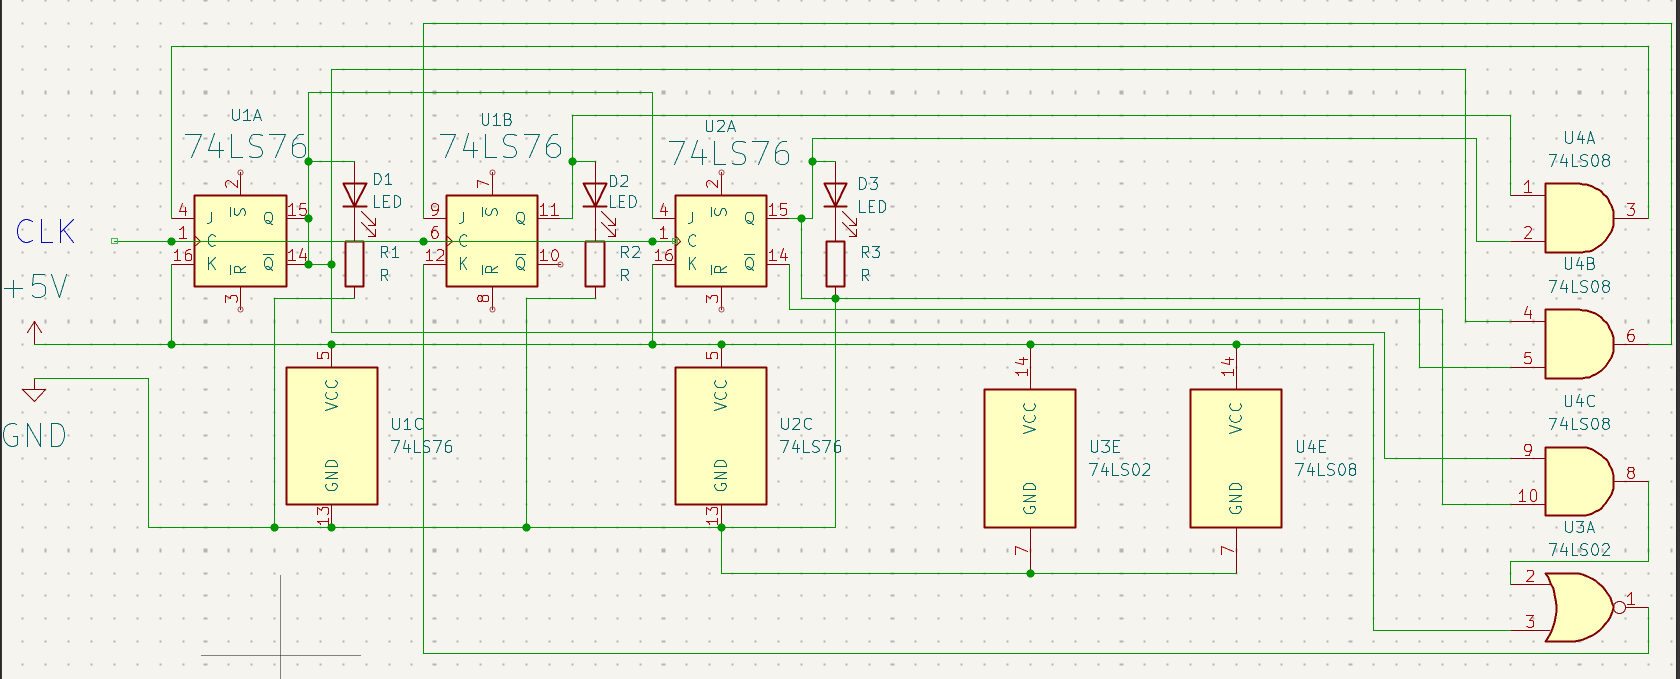
\includegraphics[width=\linewidth]{schematic.png}
    \caption{Circuit Schematic}
    \label{fig:circuit}
\end{figure}

It is also important to note that LEDs were not connected directly between Q of JK FF to GND. There was a resistor in between to limit the current flowing, so as to not destroy the LED.

\section{Observation and Debugging}

Initially, the output of the setup was restricted only to 0 and 5. It jumped from 0 to 5 and back to 0. In some cases, the circuit initialized with a state like 2 which then proceeded to 7 then back to 0.
So something like this,

$010 -> 111 -> 000 -> 101 -> 000 -> 101 -> 000 \quad...$

Naturally, our initial guess was that either the logic for the first JK FF was wrong, or we made an error while connecting the output of LED corresponding to MSB (as what should have been 001 became 101). The only expected behavior in this initial setup was the transition from 5 to 0 (101 to 000) and 7 to 0 (111 to 000) just like how we defined it in the truth table. Also initially, what should have been $010 -> 011$ became $111$, which supports our guess that the first bit was incorrect.

We hence started debugging with an Arduino UNO by connecting probes into random parts of the circuit and looking at the output in the serial monitor. The AND and NOR gates worked as expected, and so did the second and the third Flip-Flop. But there was something off about the first FF (as we initially guessed). The output Q did not match correctly with different J and K. While the logic was right and the value of $J_2$ and $K_2$ produced when the state is 000 matches with theoretical expectation, the output $Q_2$ did not match. So we assumed that the first Flip-Flop itself is not behaving as expected. We immediately checked the clear and preset pins, and they were HIGH as expected (the clear and preset pins are active-LOW). So we assumed that either the wiring for the rest of the first flip-flop isn't proper or the flip-flop itself was faulty. We hence rewired only the first flip-flop IC and also replaced it with a new one. After then fixing a few wiring mismatches, the mod 5 counter started working as expected. 

\section{Conclusion}
The LEDs were blinking in this fashion after every 1 second (clock signal was produced by AFG):
$000 -> 001 -> 010 -> 011 -> 100 -> 000$
We did not encounter any undefined state initially in this refined setup. 
We have hence successfully built a mod 5 counter with a nice representation through LEDs.

\chapter{Band Pass Filter}

\section{Objective}
A band pass filter is a filter that attenuates all frequencies other than a specific band. We build a band pass filter by cascading a low pass filter with a high pass filter. The frequency response should be centered at $15k$Hz, and we must try to extract the $15k$Hz harmonic from a $3k$Hz square wave.

\section{Calculations and setup}
The general circuit diagram for a band pass filter that works by cascading a low pass filter followed by a high pass filter is as follows:

\begin{center}
\begin{circuitikz}[american voltages]
	\draw (0, 3) 
        to[V, l_ = $v_s$](0, 0);
    \draw (0, 3)
	    to[R, l = $R_1$](3, 3)
        to[C, l_ = $C_1$](3, 0)
        -- (0, 0)
        node[ground]{};
    \draw (3, 3)
	    to[C, l = $C_2$](6, 3)
        to[R, l_ = $R_2$, v^ = $v_{out}$](6, 0)
        -- (3, 0);
\end{circuitikz}
\end{center}

\begin{align}
    \frac{v_{out}}{v_s} = \frac{1}{1+j\omega R_1C_1} \cdot \frac{j\omega R_2C_2}{1+j\omega R_2C_2}  
\end{align}

If our goal is to maximize magnitude output to input ratio at a particular frequency (in this case $15k$Hz) we differentiate the above expression w.r.t $\omega$ and set it to 0, to find maxima.
\begin{align}
    \left | \frac{v_{out}}{v_s}  \right | = \frac{1}{\sqrt{1+w^2R_1^2C_1^2}}\cdot\frac{wR_2C_2}{\sqrt{1+w^2R_2C_2}} \\
    \frac{d}{d\omega} \left ( \frac{1}{\sqrt{1+w^2R_1^2C_1^2}}\cdot\frac{wR_2C_2}{\sqrt{1+w^2R_2C_2}} \right ) = 0 \\
    \omega^2 - R_1C_1R_2C_2 = 0
\end{align}

We hence end up with, 
\begin{align}
    \omega _0 = \frac{1}{\sqrt{R_1C_1R_2C_2}}
\end{align}

Where $\omega _0$ is the angular frequency corresponding to where the frequency response is centered. We can interpret this central angular frequency as the geometric ratio of the cutoff frequencies of low-pass and high-pass filters.

Now we must choose $R_1, C_1, R_2 \text{ and }C_2$ such that $\frac{\omega_0}{2\pi} = 15k$Hz will be satisfied. 

We must also take care of the distance of the cutoff frequencies of the low-pass and high-pass component of the band pass filter. 

In this case, our goal is to design a narrow band pass filter, so we must choose the cutoff frequencies of the corresponding low and high pass filter circuits such that they are as close to each other as possible. We hence took the cutoff frequencies to be the same, i.e $R_1C_1 = R_2C_2$

So if we set $R_1C_1 = R_2C_2$, we get 
\begin{align}
    RC = \frac{1}{2\pi \times15 \times 10^3} \\
    RC = 1.06 \times10^{-5}
\end{align}

So our goal is to find corresponding values of R and C based on the resistors and capacitors available to us.
We initially considered using a $1\mu F$ capacitor with a $10\Omega$ resistor. But we then realized that the AFG itself has an impedance of $50\Omega$. This would mess up the true value of RC, and hence the frequency response would not be centered at $15k$Hz. 

So we tried to maximize R so that the $50 \Omega$ impedance would have a negligible effect on overall R. Since there weren't any capacitors with capacitances in the order of $nF$, we used the highest capacitance in the $pF$ range, which was $561pF$. We then calculated R so that $RC \approx 10^{-5}$. R came out to be $18.8 k\Omega$, which we were lucky to have. We decided to use two $18k\Omega$ resistors and two $561 pF$ capacitors in our circuit.

\begin{table}[H]
    \centering
    \begin{tabular}{|c|c|}
    \hline
        Element & Value \\
    \hline
        $R_1$ & $18k\Omega$ \\
        $C_1$ & $561pF$ \\
        $R_2$ & $18k\Omega$ \\
        $C_2$ & $561pF$ \\
    \hline
    \end{tabular}
    \caption{Resistors and Capacitors used}
    \label{tab:rescaptable}
\end{table}

\section{Circuit Diagram}

The final circuit diagram ended up looking something like this:

\begin{center}
\begin{circuitikz}[american voltages]
	\draw (0, 3) 
        to[V, l_ = $v_s$](0, 0);
    \draw (0, 3)
	    to[R, l = $18k\Omega$](3, 3)
        to[C, l_ = $561pF$](3, 0)
        -- (0, 0)
        node[ground]{};
    \draw (3, 3)
	    to[C, l = $561pF$](6, 3)
        to[R, l_ = $18k\Omega$, v^ = $v_{out}$](6, 0)
        -- (3, 0);
\end{circuitikz}
\end{center}

Terminals of AFG were used as the voltage source $v_s$. Probes of the DSO were connected between the terminals of the resistor corresponding to $v_{out}$.

\section{Output and Simulations}
\begin{figure}[H]
    \centering
    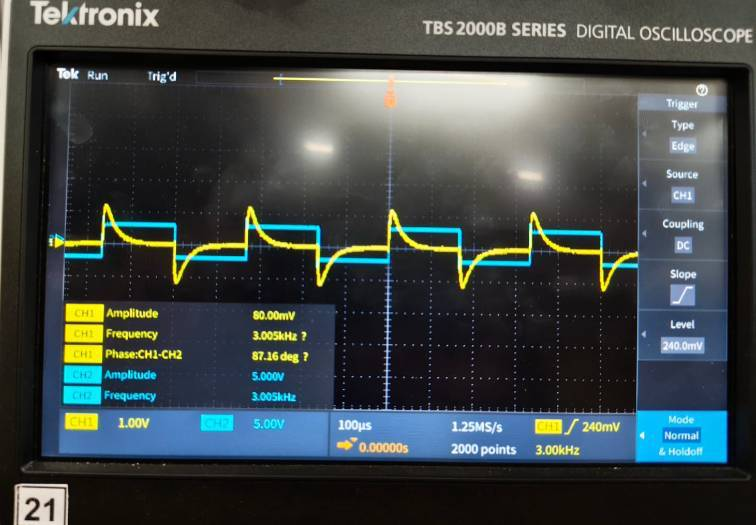
\includegraphics[width=0.8\linewidth]{timedomainresponse.jpeg}
    \caption{Output Waveform}
    \label{fig:waveform}
\end{figure}

The output waveform unfortunately did not look like a clean sine wave. We tried checking if the frequency response was centered at $15k$Hz, and it was indeed matching with the theoretical expectation. 

We simulated the output waveform, and it DID match with the experimental response. 
\begin{figure}[H]
    \centering
    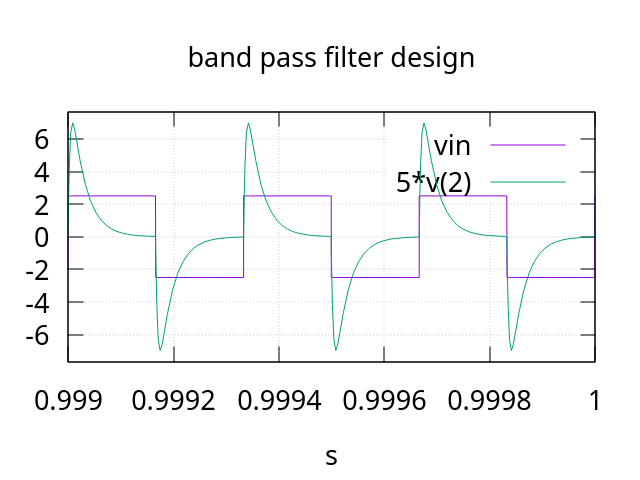
\includegraphics[width=0.5\linewidth]{bpftime.png}
    \caption{Simulated Time-Domain Response to 3kHz square wave}
    \label{fig:simulatedresponse}
\end{figure}

We also simulated the frequency response, and it was matching with the experimental results. It was centered at around $15-17 kHz$ (we used the exact resistances that we used in the experiment to simulate).
\begin{figure}[H]
    \centering
    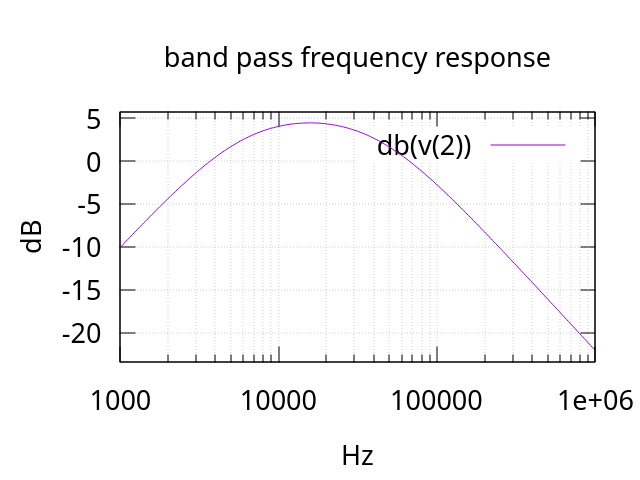
\includegraphics[width=0.5\linewidth]{bpffreq.png}
    \caption{Simulated Frequency-Domain Response}
    \label{fig:simulatedfreqresponse}
\end{figure}

\section{Observation}
In a square wave, the fourier series coefficients are given as follows
\begin{align}
    C_n = \begin{cases}
             \frac{2}{nj\pi} & \text{if n is odd} \\
            0 & \text{if n is even}
            \end{cases}
\end{align}
Note that in the equation above, n can be negative. 

So for every odd harmonic, the coefficient decays as $\frac{1}{n}$. So the $15k$Hz or the $5^{th}$ harmonic has only 1/5 weightage of the first harmonic ($3k$Hz). The band pass filter is not able to attenuate the $3k$Hz frequency enough to remove its influence. Hence the output waveform also looks like it has a frequency of $3kHz$, even though it has a good $15k$Hz component.

\section{Conclusion}
Band pass filters built by using a low pass filter followed by a high pass filter are great for attenuating frequencies other than wide bands. But in this case, where we are expected to extract only the $15kHz$ sine wave, the band pass filter failed. However we were able to get the frequency response to be centered at $15kHz$.

All the simulations are available here: 

\fbox{\parbox{\linewidth}{\url{https://github.com/Vivek-Kumar-1907/ee1200/tree/main/assignment4/simulations/}}}


\end{document}
